
% !TEX root = ../../phdthesis_tawatr.tex 
\renewcommand{\thisdir}{_content/reg1d_synthetic_3d}
\renewcommand{\figdir}{\thisdir/_fig}

%% ==== ==== ==== ====
\section[3D examples]{Estimating a model of regional mean 1D profile: 3D example}\label{sect:example_3d}

%% ==== Model 3D plane view
\begin{figure}[!b]
	\centering
	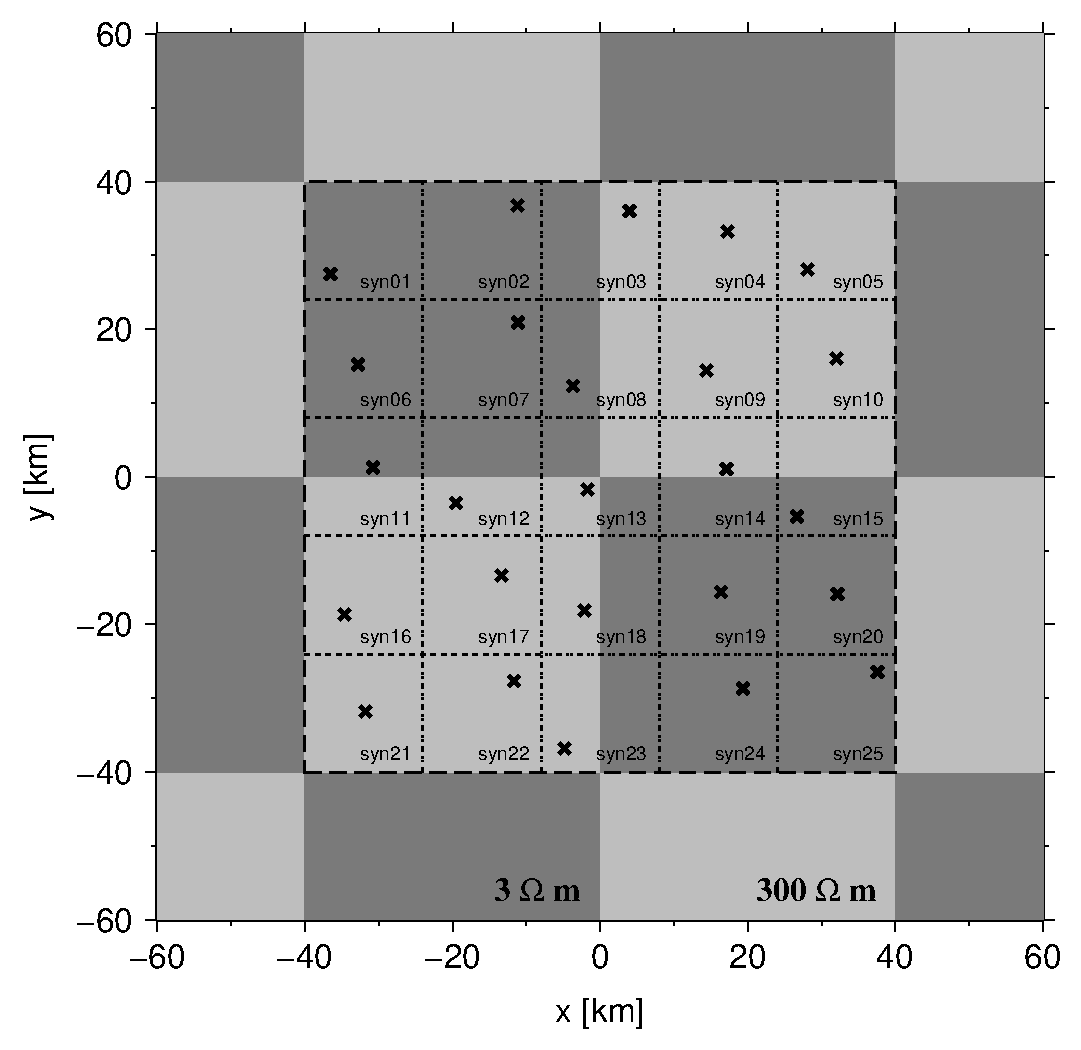
\includegraphics[width=\plotchkboardsize]{\figdir/m02a_chkboard12_h0a2a_s40k_p0p0_pp1.pdf}
	\caption[Checkerboard model and MT array setting used in this study]{Model of checkerboard anomalies with resistivities of 3 and 300 {\Ohmm} and a size of  \areakm{40}{40} embedded in the lower crust layer. The array of 25 irregularly distributed MT stations (crosses) covers the area of interest, which is {\areakm{80}{80}} (dashed frame). Here, one MT station represents an area of {\areakm{16}{16}} (dash-dotted frames).}
	\label{fig:model3d_setting}
\end{figure}

%% ==== 
The 3D model used in this work are generated from embedding checkerboard anomalies with resistivities of 3 and 300 {\Ohmm} and a size of \areakm{40}{40} (Figure \ref{fig:model3d_setting}) in the lower crust (14.8--33.3 km depth) of the layered-Earth model as in the 1D example (Figure \ref{fig:lyrearth_model}). The anomalies at this depth range could be detectable within the given period range.
% 
We can determine the inductive scale length using Eq. \eqref{eq:idl_anomaly}, where the conductivity contrast $\delta \sigma$ is $1/3 - 1/300$ Sm$^{-1}$. From the shortest to the longest periods (1--1,000 s), the inductive scale lengths corresponding to these anomalies range from 876 m to 27.7 km. They are not much smaller than its physical dimension (\areakm{40}{40}); therefore, the inductive effect from these anomalies should be sufficient.

%% ==== 
The details of the MT array configuration are as follows. The 25 MT stations are distributed over the area of interest which is \areakm{80}{80} (Figure \ref{fig:model3d_setting}). Consequently, the site spacing is 16 km, i.e., each site represents an area of \areakm{16}{16} (1/25 of the area of interest). To simulate the irregularly distributed MT array, the location of the $i$th station is given by
\begin{equation*}
	\begin{split}
		x_i & = x_c + s r_x \\
		y_i & = y_c + s r_y, \\
	\end{split}
\end{equation*}
where $(x_c,y_c)$ is the coordinate of the mesh center represented by each MT site; $s$ is the site spacing, which is 16 km in the setup; $r_x$ and $r_y$ are uniform random numbers bounded within $(-0.5,+0.5)$.

%% ==== Figure: 3D response individual all (undistorted)
\begin{figure}[!b]
	\centering
	\subfigure[]{
		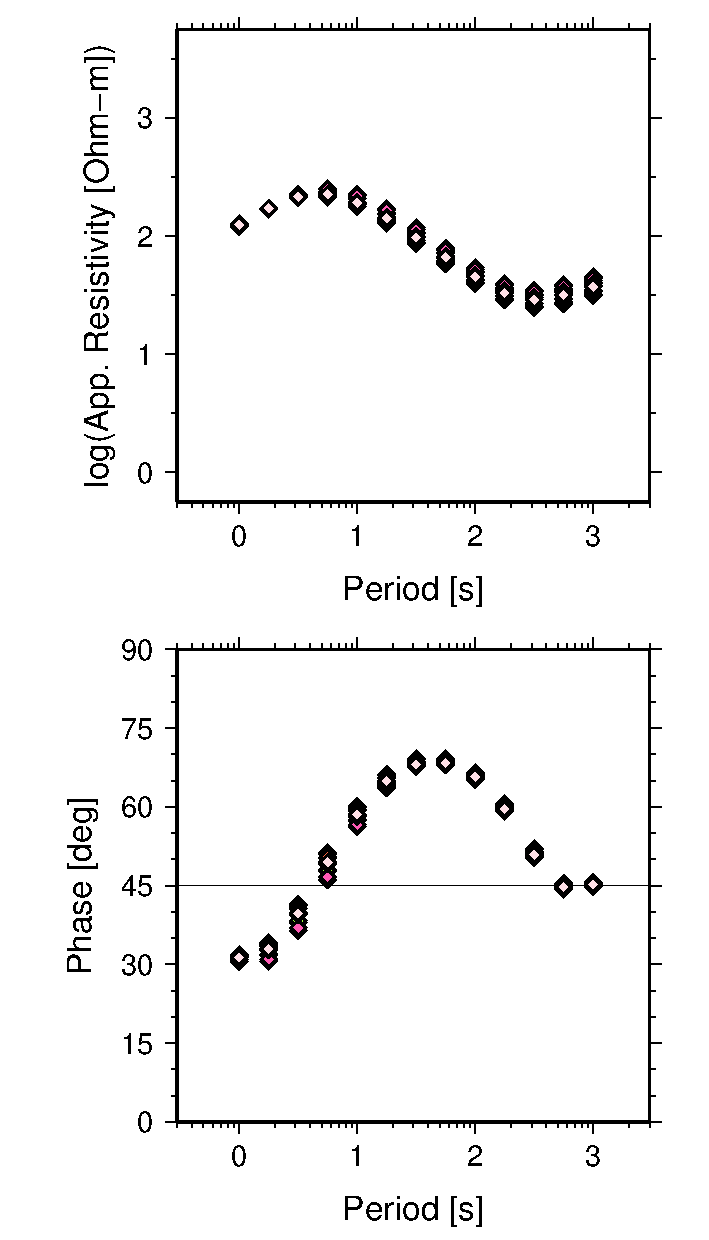
\includegraphics[scale=\plotmtrespscale]{\figdir/m02a-lyr11a_cb12-h0a2a-d05a-t01a_dr-e43n42_cb1X_loc-regi0_c-s40k-p0p0-pp1_d13a_undistorted_zinv_det_arsphs.pdf}
		\label{fig:resp3d_individual_all_undistorted_det}
	}
	\subfigure[]{
		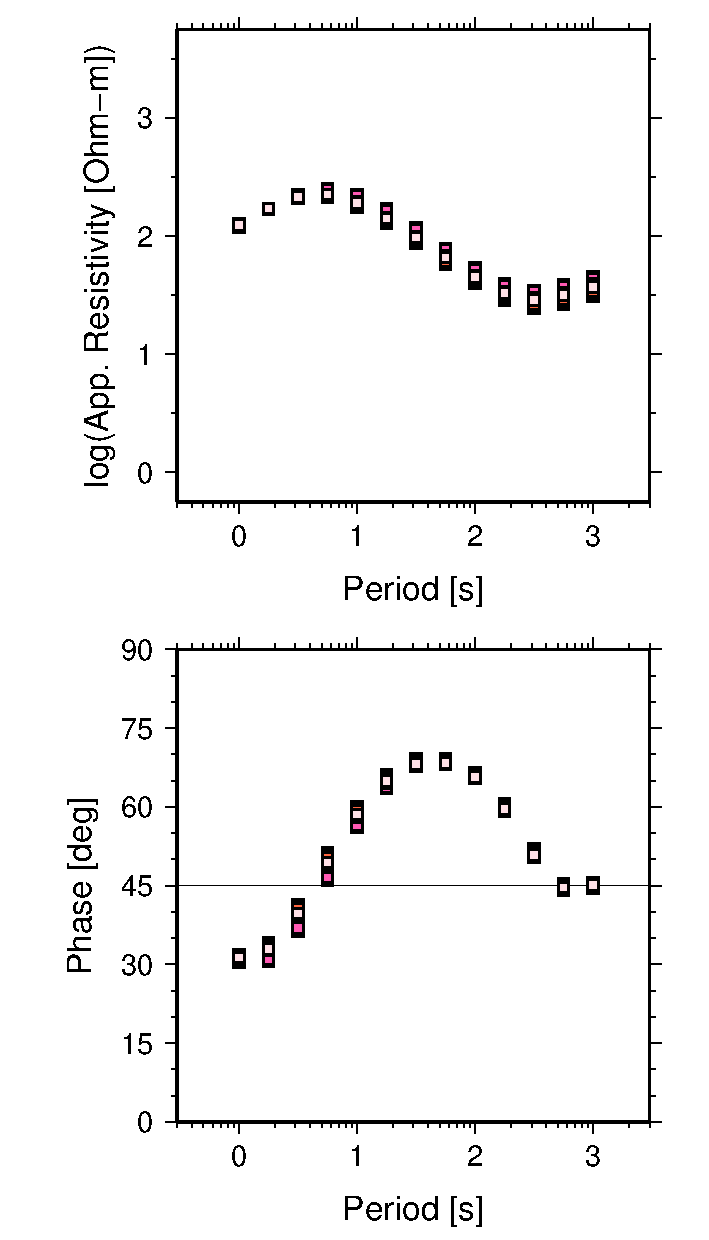
\includegraphics[scale=\plotmtrespscale]{\figdir/m02a-lyr11a_cb12-h0a2a-d05a-t01a_dr-e43n42_cb1X_loc-regi0_c-s40k-p0p0-pp1_d13a_undistorted_zinv_ssq_arsphs.pdf}
		\label{fig:resp3d_individual_all_undistorted_ssq}
	}
	\caption[Det and ssq impedances from MT array over the checkerboard model]{(a) Det and (b) ssq impedances from the array of MT stations over the 3D anomalies. Each station is represented by a different symbol color.}
	\label{fig:resp3d_individual_all_undistorted}
\end{figure}


%% ==== 
The MT responses are calculated using the software WSINV3DMT \citep{siripunvaraporn2005a}.  
%
Without galvanic distortion, the static shift is not observed in the det and ssq impedances, and their distributions are also similar (Figure \ref{fig:resp3d_individual_all_undistorted}). 
%
The checkerboard anomalies are recognized in the period range of 2--30 s, as seen from the slight variation in the impedances. 
%
To obtain the distorted 3D dataset, the set of random distortion parameters as used in the 1D example were applied to the calculated 3D data using Eq. \eqref{eq:z_distorted}. 
%
The example of the undistorted MT impedance from the station \texttt{syn08} is shown in Figure \ref{fig:resp3d_example_zij_undistorted}. The magnitudes of the diagonal components -- $xx$ and $yy$ -- are rather weak.
When it is distorted, their magnitudes increase (Figure \ref{fig:resp3d_example_zij_distorted}), and
 the phase mixing, i.e., the frequency dependent feature of the $xx$ phase, can be observed.
%
Unlike the 1D case, the ssq impedance from the distorted impedances is not only shifted, but also contains a weak frequency dependence (Figure \ref{fig:resp3d_example_distorted_zinv}), which is better observed from the difference of the magnitude and phase between the distorted and undistorted rotational invariants (Figure \ref{fig:resp3d_example_distorted_zinvdiff}).
As shown before, the phase of det impedance is not altered by galvanic distortion (Figure \ref{fig:resp3d_example_distorted_zinvdiff}), but its magnitude is biased downward due to the shear and splitting parameters as with the det impedance from the distorted 1D data.


%% ==== Figure: Distored 3D response example
\begin{figure}[t]
	\centering
	\subfigure[]{
		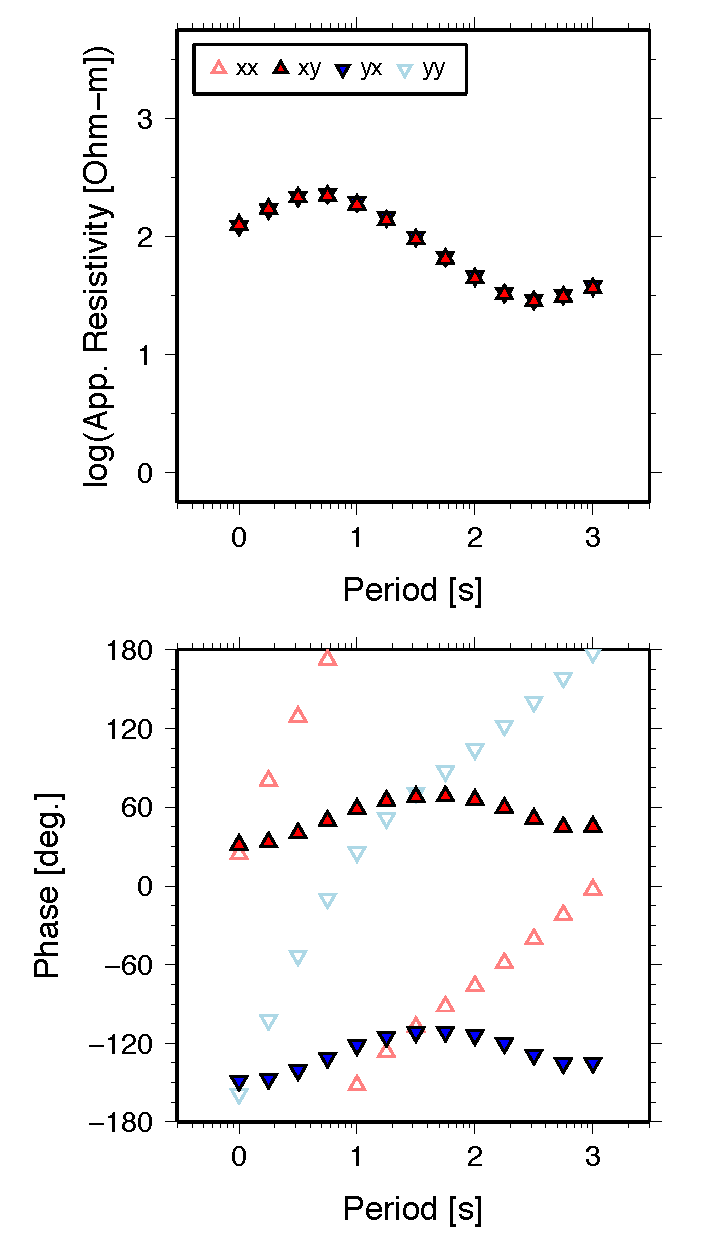
\includegraphics[scale=\plotmtrespscale]{\figdir/syni0203-azm000_zij_arsphs_undistorted.pdf}
		\label{fig:resp3d_example_zij_undistorted}
	}
	\subfigure[]{
		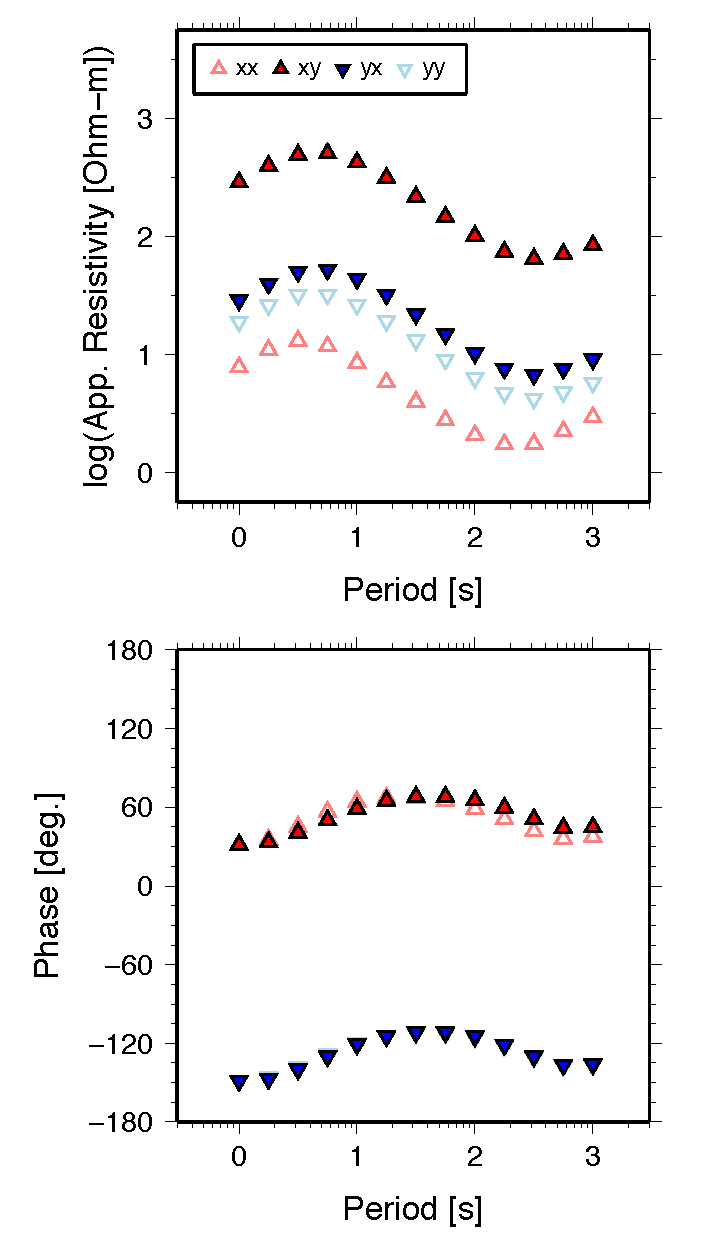
\includegraphics[scale=\plotmtrespscale]{\figdir/syni0203-azm000_zij_arsphs_distorted.pdf}
		\label{fig:resp3d_example_zij_distorted}
	}
	\caption[Examples of undistorted and distorted 3D MT data]{Components of the MT impedance from station \texttt{syn08} (a) undistorted and (b) distorted with $(g,t,e,s) = (1.20,0.11,-0.37,0.49)$.}
	\label{fig:resp3d_example_zij}
\end{figure}

%\redb{Individual from SD=0.3 and average}

As with the 1D example, the main feature observed from the det and ssq impedances due to the effect of random galvanic distortion paramters is an irregular shift (Figure \ref{fig:resp3d_individual_all_distorted_sd3a}). 
The advantage of using the ssq impedances is evident when they are averaged (Figure \ref{fig:resp3d_avg_distorted}). 
The error bar here is also the standard deviation.
As with the 1D example, the average ssq impedances has a smaller error bar smaller than the average det impedances at the same strength of galvanic distortion. 
This supports the idea that the ssq impedance is less dispersed due to galvanic distortion. 
Also, the average det impedances is biased downward by the splitting and shear parameters.

%% ==== Figure: Distored 3D response example inv
\begin{figure}[t]
	\centering
	\subfigure[]{
		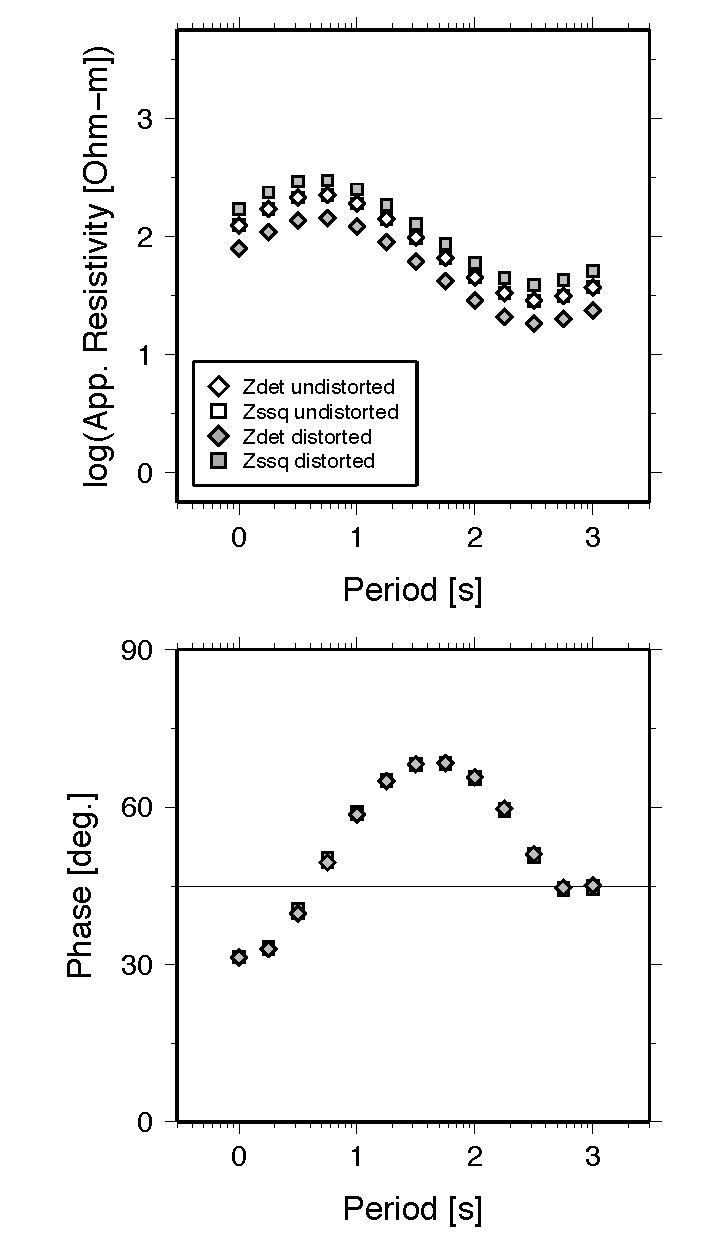
\includegraphics[scale=\plotmtrespscale]{\figdir/m02a-lyr11a_cb12-h0a2a-d05a-t01a_dr-e43n42_cb1X_loc-regi0_c-s40k-p0p0-pp1_d13a_syni0203_zinv_arsphs.pdf}
		\label{fig:resp3d_example_distorted_zinv}
	}
	\subfigure[]{
		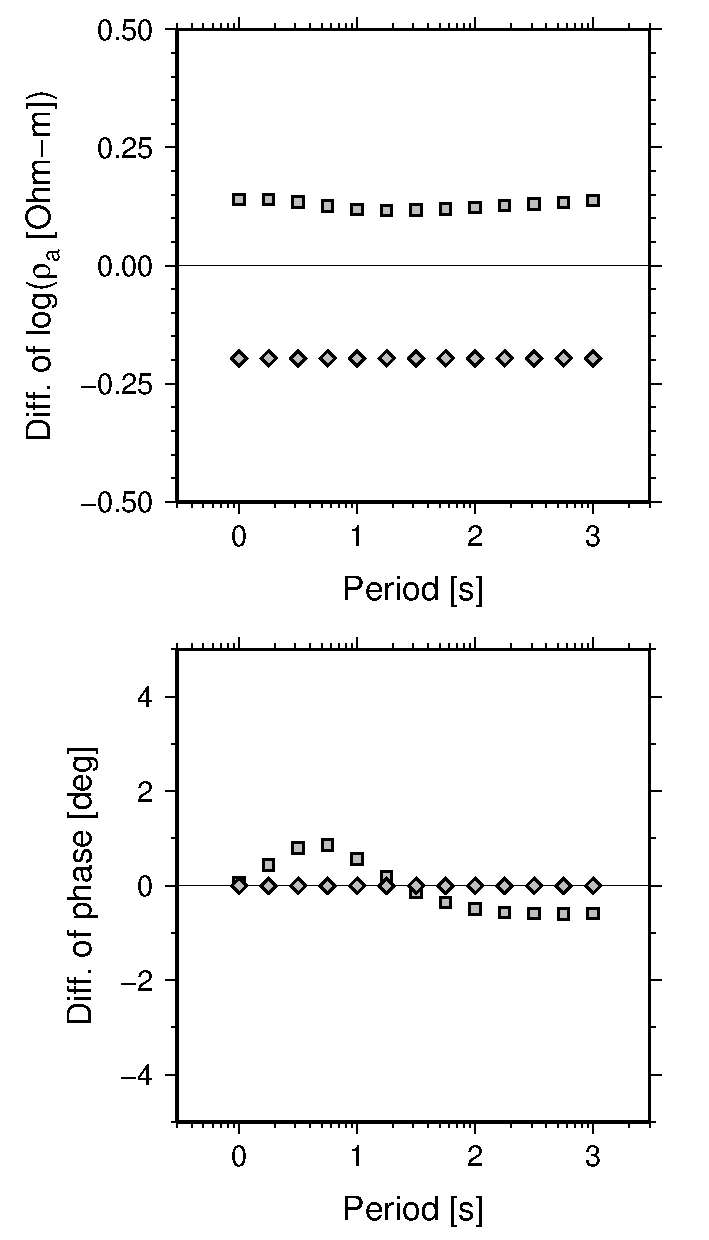
\includegraphics[scale=\plotmtrespscale]{\figdir/m02a-lyr11a_cb12-h0a2a-d05a-t01a_dr-e43n42_cb1X_loc-regi0_c-s40k-p0p0-pp1_d13a_syni0203_zinvdiff_arsphs.pdf}
		\label{fig:resp3d_example_distorted_zinvdiff}
	}
	\caption[Det and ssq impedances derived from the undistorted and distored MT impedance]{(a) Corresponding det and ssq impedances of the undistorted and distorted impedances in Figure \ref{fig:resp3d_example_zij}. (b) Difference between distorted and undistorted rotational invariant impedances.}
	\label{fig:resp3d_example_distorted}
\end{figure}

%\redb{Inverted model}

To yield the models of the regional mean 1D conductivity profile, the average distorted det and ssq impedances are inverted with the same uncertainty and convergence condition as used in the 1D example.
%
Without galvanic distortion, the average det and ssq impedances results in very similar models (Figure \ref{fig:resp3d_avg_distorted_model}).
The models estimated from the undistorted data both det and ssq impedances seem consistent with the theoretical models, which is obtanied by applying Eqs. \eqref{eq:regional_mean_linear} and \eqref{eq:regional_mean_log} to the conductivity distribution within the area of interest (dashed frame in Figure \ref{fig:model3d_setting}).
The discussion of the theoretical model is given in Section \ref{sect:reg1d_exam}.
%
As with the 1D example, when the galvanic distortion is included, the average det impedances will give the more conductive models of the regional mean 1D conductivity profile. On the contrary, using the average ssq impedances results in the models that are close to the model derived from the undistorted cases at any galvanic distortion strength.
This result strongly supports the idea that the average ssq impedance is an promising parameter in estimating the model of the regional mean 1D conductivity profile.





%% ==== Model 3D inverted individual
%\begin{figure}
%	\centering
%	\includegraphics[height=4in]{path1}
%	\caption{caption1}
%	\label{fig:caption1}
%\end{figure}


%\missingfigure[figwidth=6cm]{Figure showing 1D inverted from station over different underlying structure}



%% ==== Figure: Distored 3D response individual all
\begin{figure}[t]
	\centering
	\subfigure[]{
		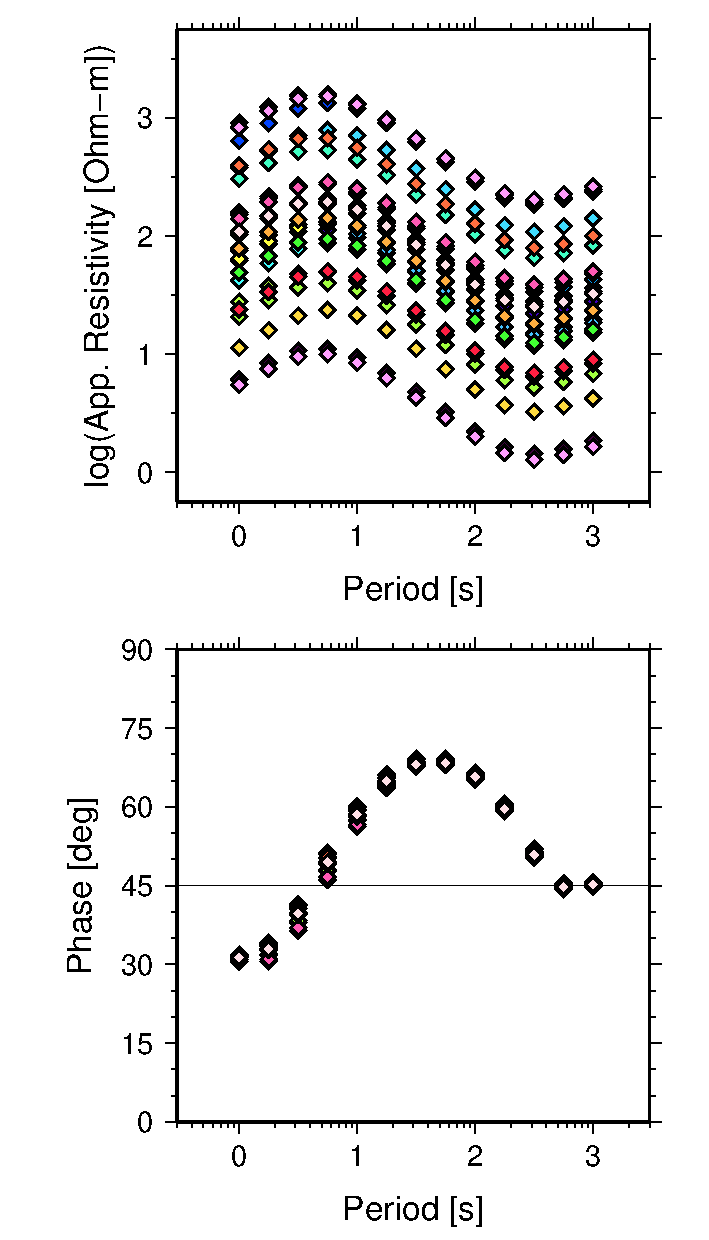
\includegraphics[scale=\plotmtrespscale]{\figdir/m02a-lyr11a_cb12-h0a2a-d05a-t01a_dr-e43n42_cb1X_loc-regi0_c-s40k-p0p0-pp1_d13a_distorted-sd3a-gtes_zinv_det_arsphs.pdf}
		\label{fig:resp3d_individual_all_distorted_sd3a_det}
	}
	\subfigure[]{
		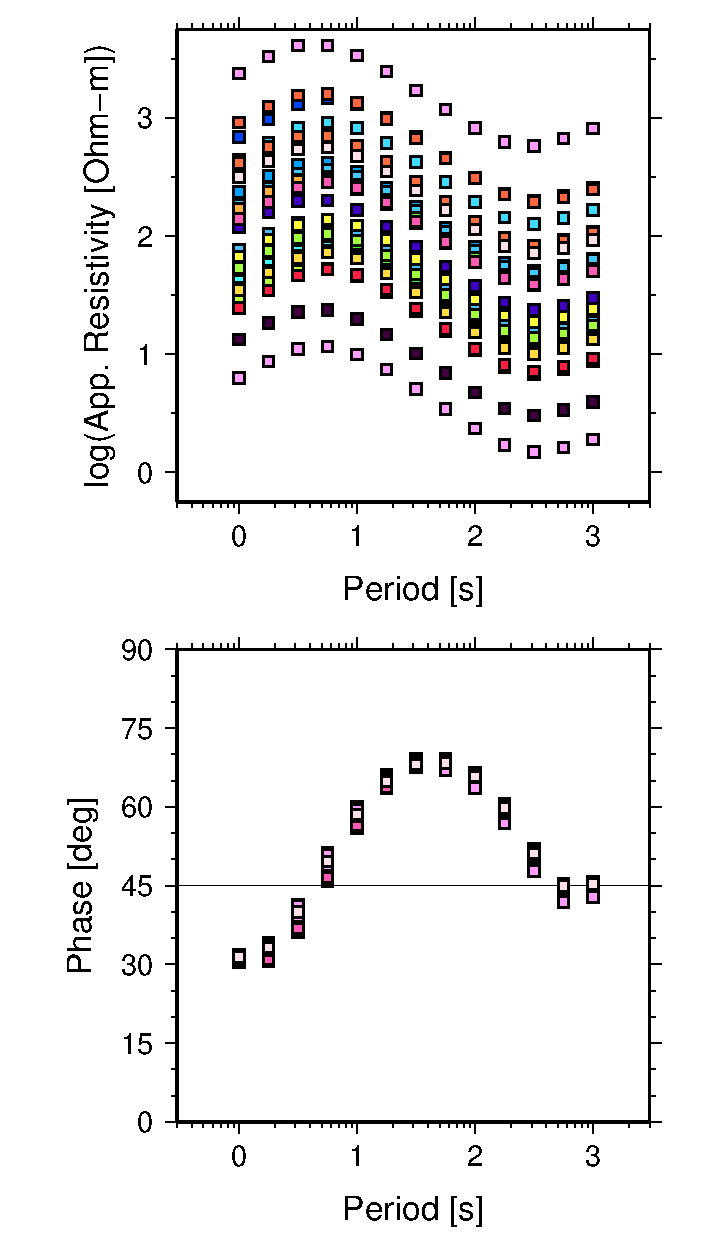
\includegraphics[scale=\plotmtrespscale]{\figdir/m02a-lyr11a_cb12-h0a2a-d05a-t01a_dr-e43n42_cb1X_loc-regi0_c-s40k-p0p0-pp1_d13a_distorted-sd3a-gtes_zinv_ssq_arsphs.pdf}
		\label{fig:resp3d_individual_all_distorted_sd3a_ssq}
	}
	\caption[Example of distorted det and ssq impedances from distorted 3D MTdataset]{(a) Det and (b) ssq impedances from the 3D example (as shown in Figures \ref{fig:resp3d_individual_all_undistorted_det} and \ref{fig:resp3d_individual_all_undistorted_ssq}, respectively) where a set of distortion parameters with an SD of 0.3 was applied.}
	\label{fig:resp3d_individual_all_distorted_sd3a}
\end{figure}

%% ==== Figure: Distored 3D response average
\begin{figure}[t]
	\centering
	\subfigure[]{
		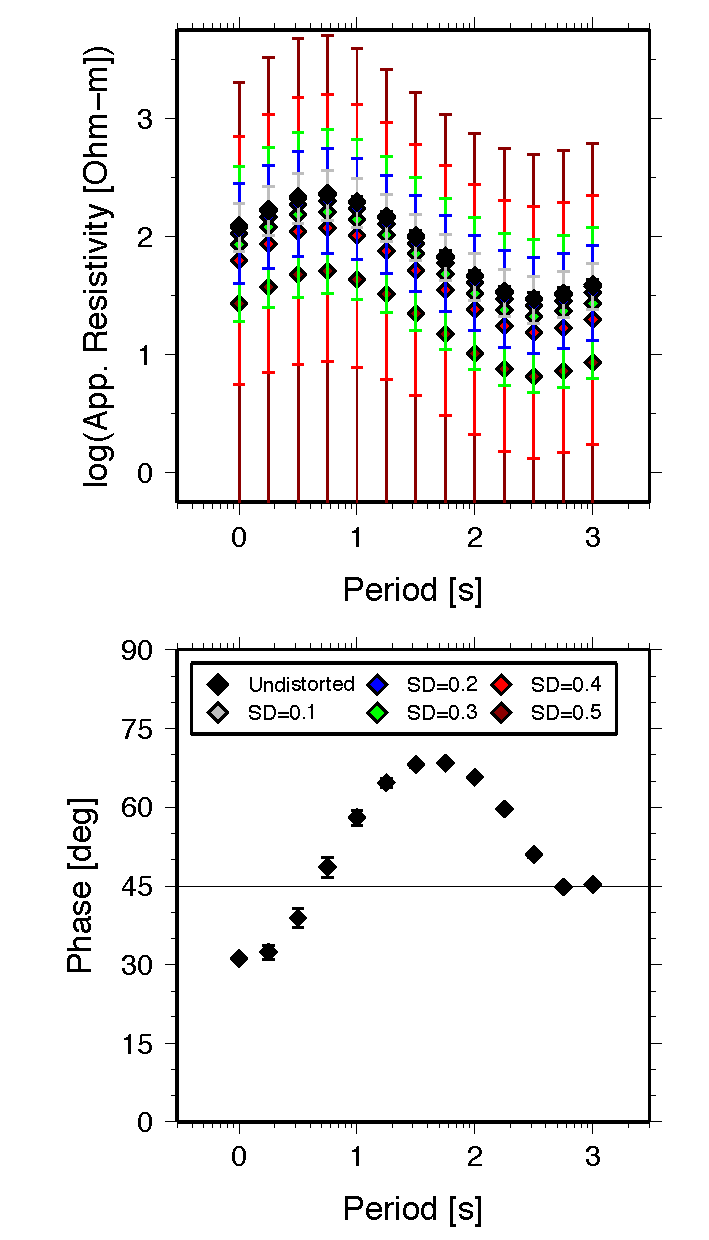
\includegraphics[scale=\plotmtrespscale]{\figdir/m02a-lyr11a_cb12-h0a2a-d05a-t01a_dr-e43n42_cb1X_loc-regi0_c-s40k-p0p0-pp1_d13a_distorted-sdxa_site_dispsd_zinv_det_arsphs.pdf}
		\label{fig:resp3d_avg_distorted_det}
	}
%	\hspace{1cm}
	\subfigure[]{
		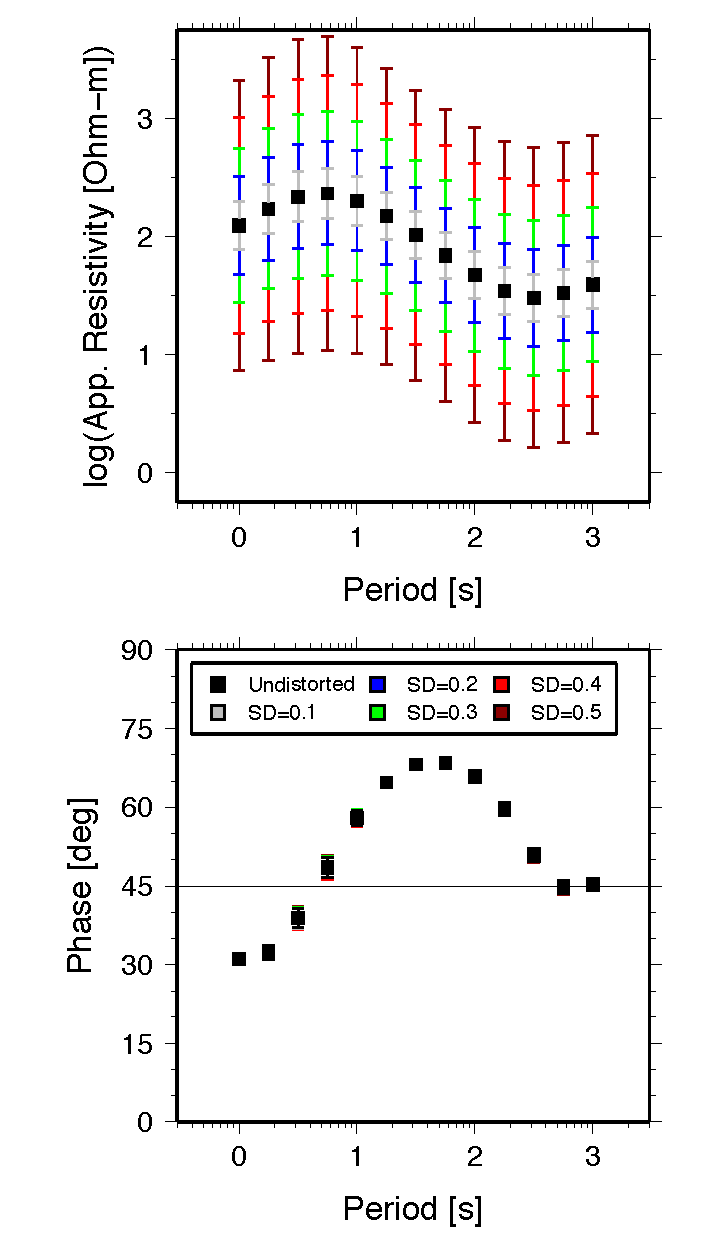
\includegraphics[scale=\plotmtrespscale]{\figdir/m02a-lyr11a_cb12-h0a2a-d05a-t01a_dr-e43n42_cb1X_loc-regi0_c-s40k-p0p0-pp1_d13a_distorted-sdxa_site_dispsd_zinv_ssq_arsphs.pdf}
		\label{fig:resp3d_avg_distorted_ssq}
	}
	\caption[Average det and ssq impedances from 3D MT datasets distorted
with different galvanic distortion strengths]{Average (a) det and (b) ssq impedances from the 3D datasets distorted with different galvanic distortion strengths.}
	\label{fig:resp3d_avg_distorted}
\end{figure}

%% ==== Figure: Distored 3D response average inverted
\begin{figure}[t]
	\centering
	\subfigure[]{
		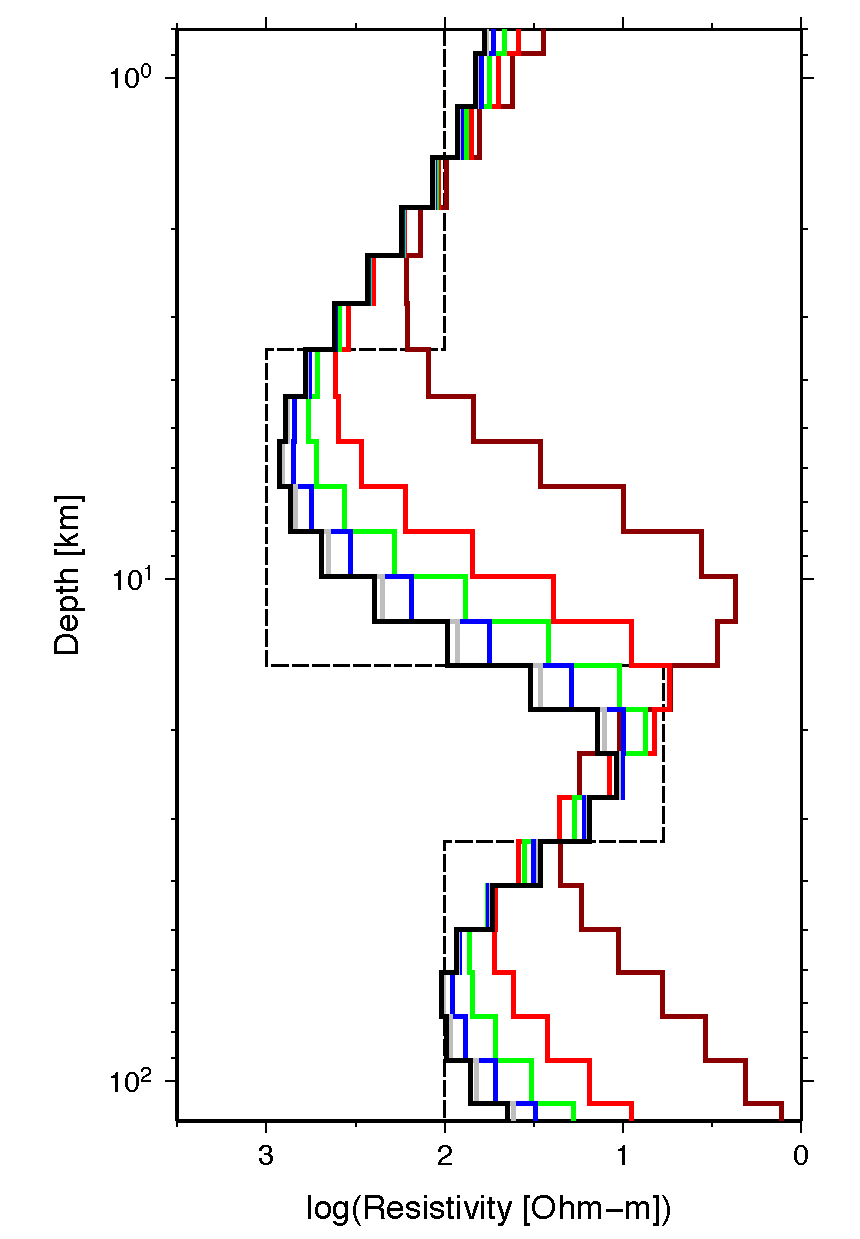
\includegraphics[scale=\plotinvmodelscale]{\figdir/m02a-lyr11a_cb12-h0a2a-d05a-t01a_dr-e43n42_cb1X_loc-regi0_c-s40k-p0p0-pp1_d13a_distorted-sdxa_site_dispse_det.pdf}
		\label{fig:resp3d_avg_distorted_model_det}
	}
	\subfigure[]{
		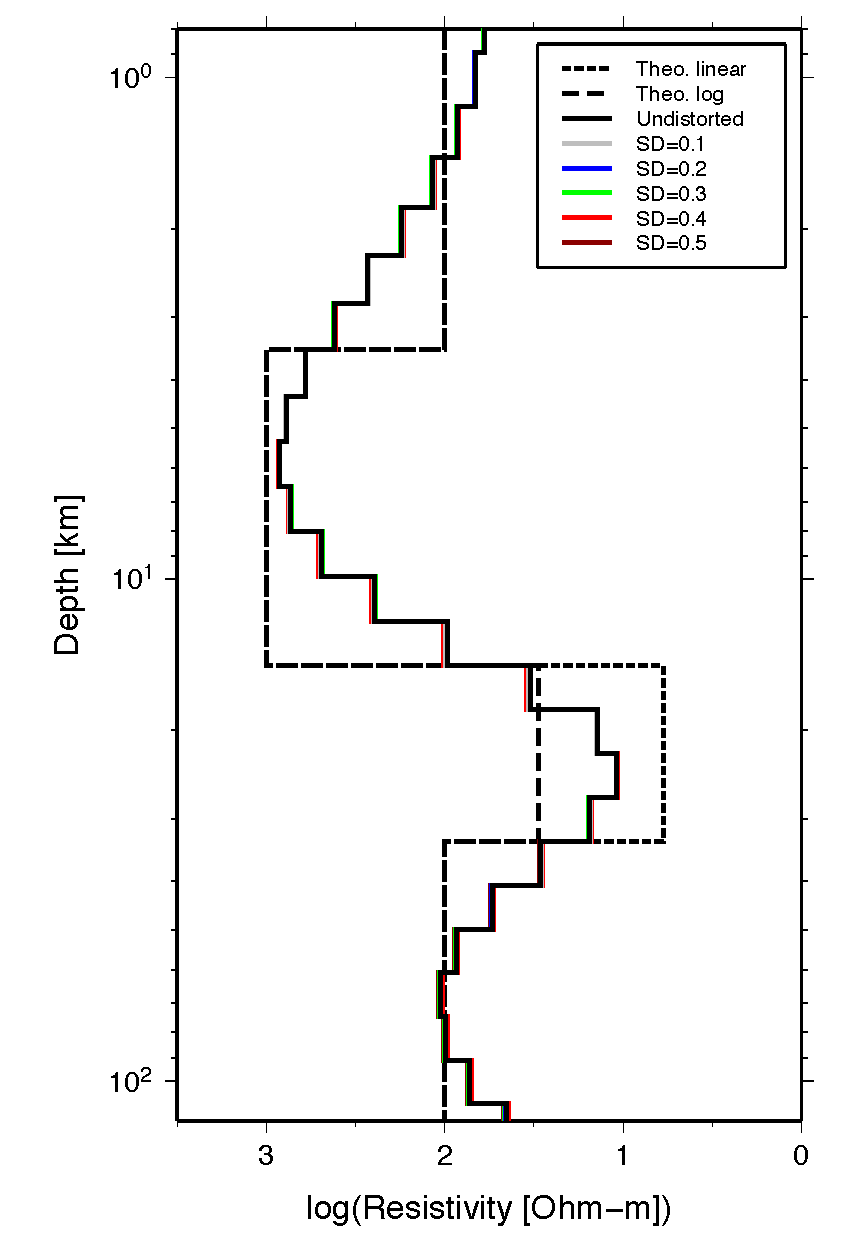
\includegraphics[scale=\plotinvmodelscale]{\figdir/m02a-lyr11a_cb12-h0a2a-d05a-t01a_dr-e43n42_cb1X_loc-regi0_c-s40k-p0p0-pp1_d13a_distorted-sdxa_site_dispse_ssq.pdf}
		\label{fig:resp3d_avg_distorted_model_ssq}
	}
	\caption[Inverted models from average det and ssq impedances from distorted 3D datasets]{1D models inverted from the average (a) det and (b) ssq impedances from the distorted 3D datasets (Figure \ref{fig:resp3d_avg_distorted}). The theoretical model of the mean 1D profile from this setting is shown for comparison.}
	\label{fig:resp3d_avg_distorted_model}
\end{figure}
